\chapter{Теоретичні відомості}\label{chapter2}
Другий розділ присвячено опису ефекту бінокулярного стереозору, постановці та розв'язку задачі стереозору для випадку повних даних.

%%===========================================================================%%
\section{Знаходження глибини методом бінокулярного паралаксу}
%%===========================================================================%%
\subsection{Будова камери}
Сучасні цифрові фото та відео камери мають куди більш складну будову, ніж їх попередники. Для подальших викладок нам буде достатньо розглянути роботу найпростішої можливої камери --- камери-обскури (від лат. camera obscūra --- «темна кімната») (рис. \ref{1.1.1 - Camera-obscura}). Це просто темне приміщення з одним малим отвором (його називають \textit{точковою діафрагмою}), через який на протилежну стіну проектується перевернуте зображення предметів ззовні. Для нас протилежна стіна --- матриця цифрової камери. 
\begin{figure}[H]
	\centering
	\includegraphics[scale = 0.5]{CO2.pdf}
	\caption{Будова камери-обскури.\\ 1 --- результуюче зображення, 2 --- отвір, 3 --- віртуальне зображення, 4 --- об'єкт}
	\label{1.1.1 - Camera-obscura}
\end{figure}


%%---------------------------------------------------------------------------%%
\subsection{Пошук відстані методом бінокулярного паралаксу}
В силу оптичних особливостей результуюче зображення в камерi-обскурі буде перевернутим. Тому замість нього будемо розглядати віртуальне зображення, що знаходиться на відстані $f$ з права від діафрагми, але вже не перевернуте (рис. \ref{1.1.1 - Camera-obscura}).
Це ніяк не вплине на результат, але спростить подальші викладки.
Покажемо тепер, як з допомогою двох таких камер можна знайти абсолютну відстань до об'єкта. Камери розташовані паралельно одна одній.
Тоді маємо таку конфігурацію (рис. \ref{geometry}). Тут $L$ та $R$ --- діафрагми лівої та правої камери, $O_L, O_R$ --- центри віртуальних зображень,
\begin{figure}[!htb]
	\centering
	\includegraphics[scale = 0.6]{geometry.pdf}
	\caption{Геометрія розташування камер.}
	\label{geometry}
\end{figure}
$f$ --- фокусна відстань, $z$ --- відстань до об'єкта, $\Delta$ --- відстань між камерами, $x_1$ та $x_2$ --- координати проекцій об'єкта на лівому та правому зображеннях, $S$ --- об'єкт.

Тоді з подібності трикутників $LSL' , Lx_1O_L$ та $RSR' , Rx_2O_R$ маємо
$$\begin{cases} \frac{f}{x_1} = \frac{z}{\Delta + x} , \\ \frac{f}{x_2} = \frac{z}{x} . \end{cases}$$
	
Виразивши $\Delta$ з першого рівняння та $x$ з другого, отримаємо
$$\begin{cases} \Delta = \frac{z \cdot x_1}{f} - x , \\ x = \frac{z \cdot x_2}{f} . \end{cases}$$
	
Підставимо $x$ в перше рівняння і отримаємо вираз для $z$
$$ z = \frac{\Delta \cdot f}{(x_1 - x_2)} .$$
	
Оскільки $\Delta$ и $f$ не залежать від розташування об'єкта, то відстань до нього буде залежати тільки від різниці $x_1 - x_2$, тобто тільки від зсуву проекцій об'єкту між двома знімками. Тож для знаходження глибини сцени нам необхідно знайти зсув для кожного пікселя між зображеннями.
	


%%===========================================================================%%
\section{Оффлайн алгоритм пошуку скалярного поля зсувів}\label{offline}
%%===========================================================================%%
\subsection{Постановка задачі}
Нехай $n$ --- довжина зображення, $I = \{1, 2, .., n\}$ --- множина координат пікселів, $D = \{0, ... , D_{max}\}$ ---  множина зсувів, де $D_{max}$ --- значення максимального зсуву, що обирається емпіричним шляхом. 
Ліве і праве зображення задамо як функції
\begin{align*}
	\mathcal{L} &: I \rightarrow \mathcal{C} , \\
	\mathcal{R} &: I \rightarrow \mathcal{C} .
\end{align*}
Тобто, $\mathcal{L}(i)$ --- інтенсивність $i$-го пікселя на лівому зображені, а $\mathcal{R}(i)$ --- інтенсивність $i$-го пікселя на правому зображені, а $ \mathcal{C} $ --- множина кольорів зображення.

Для вирішення задачі кожному пікселю лівого зображення потрібно знайти відповідний йому піксель на правому зображенні (\ref{mapping}). Введемо сюр'єктивне відображення $ d : I \rightarrow D $, де $ d(i) $ --- такий зсув $ d_i \in D$ для пікселя з номером $i$ лівого зображення, що піксель правого зображення  з номером $i - d_i$ відповідає йому.
%mapping
\begin{figure}[h!]
	\centering
	\includegraphics[scale = 1]{mapping.pdf}
	\caption{Пошук відповідних пікселів}
	\label{mapping}
\end{figure}
Проте, не будь-яка пара пікселів може знаходитися у відповідності --- пікселю з номером $i$ на лівому зображені можуть відповідати пікселі  правого зображення з номером $j$, для яких $i \geq j$. Переконатися в цьому можна, тримаючи перед собою олівець, та по черзі закриваючи то праве, то ліве око. Для правого ока олівець буде знаходитися лівіше ніж для лівого

Треба знайти таку послідовність $\overline{d} \in {D}^n$, яка мінімізує штрафну функцію
\begin{equation}
	\mathcal{W}(\overline{d}) = \sum\limits_{i = 1}^n h(i, d_i) + \sum\limits_{i = 1}^{n-1} g(d_i, d_{i + 1}),
	\label{penalty}
\end{equation}
де $ h(i, d_i) $ відповідає за схожість кольору пікселів, а $ g(d_i, d_{i + 1}) $ за гладкість поля зсувів.


%%---------------------------------------------------------------------------%%
\subsection{Представлення задачі як пошук найкоротшого шляху у графі}\label{offline_graph}
Зведемо задачу пошуку послідовності $ \overline{d} $ , що мінімізує штрафну функцію \eqref{penalty}, як пошук найкоротшого шляху через орієнтований зважений граф $G = <\mathcal{V}, \mathcal{E}>$ (рис. \ref{graphG}).
Його множина вершин 
$$ \mathcal{V} = \{ \sigma(i, d) \, | \, i \in I, \, d \in D \} \cup \{ S, E \} .$$
Введемо функцію ваг вершин
\begin{align*}
v : \mathcal{V} \setminus \{S&, E\} \rightarrow \mathbb{R},\\
v(\sigma(i,d)) = h(i,d)&, \; \forall i \in I, \, d \in D . 
\end{align*}
Множина його ребер
$$ \mathcal{E} = \bigcup\limits_{d \in D } \{ <S, \sigma(1, d) > \} \; \cup \bigcup\limits_{\substack{d \in D}} \{ <\sigma(n, d), E > \} \; \cup 
\bigcup\limits_{\substack{i = 1..n-1 \\d \in D \\d' \in D}} \{ <\sigma(i, d), \sigma(i+1, d') > \} .$$
Введемо функцію ваг ребер 
$$ w : \mathcal{E} \rightarrow \mathbb{R}, $$
де $ w(v_1, v_2) $ ---  вага ребра $ <v_1, v_2>, \; <v_1, v_2> \in \mathcal{E} $,
\begin{align*}
w(\sigma(i, d), \sigma(i + 1, d ') ) &= g(d, d'), \; \forall d, d' \in D, i \in I,\\
w(S,  \sigma(1, d) ) &= 0 ,  \forall d \in D,\\
w(\sigma(n, d), E ) &= 0 ,  \forall d \in D.
\end{align*}

\newpage
\begin{figure}[t]
	\centering
	\tikzset{>=latex}
	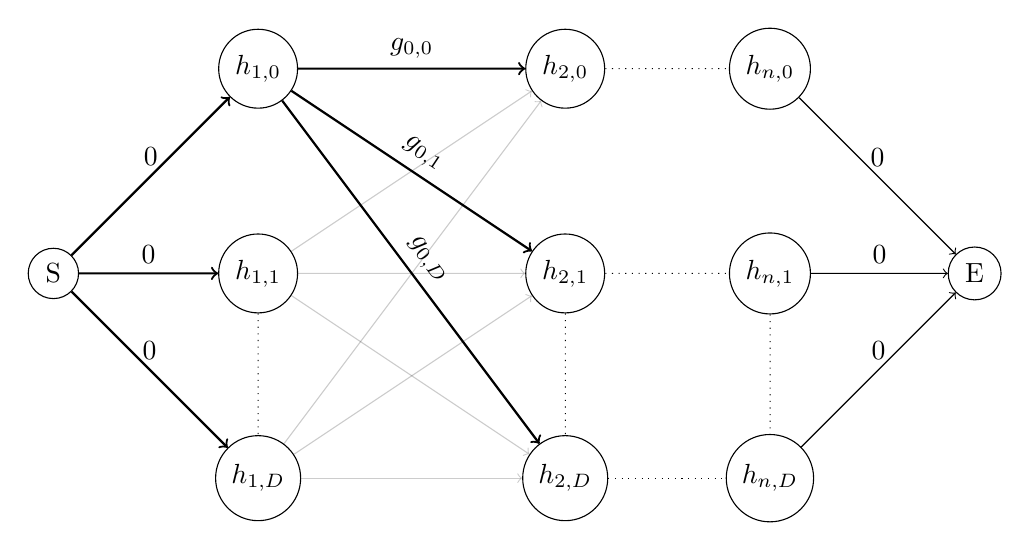
\begin{tikzpicture}[scale=1.3]
	\tikzstyle{vertex} = [circle, draw=black]
	\tikzstyle{edge} = [->, thick]

%----------Виходить такий граф:------------------------------
	\node[vertex] (s) at (0,2) {S};
	
	\node[vertex] (v1n) at (2,0) {$h_{1,D}$};
	\node[vertex] (v11) at (2,2) {$h_{1,1}$};
	\node[vertex] (v10) at (2,4) {$h_{1,0}$};
	
	\path[->, thick] (s) edge node[ above ] {0} (v1n);
	\path[->, thick] (s) edge node[ above ] {0} (v11);
	\path[->, thick] (s) edge node[ above ] {0} (v10);
	
	\draw[dash pattern=on \pgflinewidth off 2pt] (v11)--(v1n);
	
%------------------------------------------------------------
	\node[vertex] (v2n) at (5,0) {$h_{2,D}$};
	\node[vertex] (v21) at (5,2) {$h_{2,1}$};
	\node[vertex] (v20) at (5,4) {$h_{2,0}$};

	\path[->, opacity=0.2] (v11) edge node[ above,sloped ] {} (v2n);
	\path[->, opacity=0.2] (v11) edge node[ above,sloped ] {} (v21);
	\path[->, opacity=0.2] (v11) edge node[ above,sloped ] {} (v20);
	
	\path[->, opacity=0.2] (v1n) edge node[ above,sloped ] {} (v2n);
	\path[->, opacity=0.2] (v1n) edge node[ above,sloped ] {} (v21);
	\path[->, opacity=0.2] (v1n) edge node[ above,sloped ] {} (v20);
	
	%Selected
	\path[->, thick] (v10) edge node[ above,sloped ] {$g_{0,D}$} (v2n);
	\path[->, thick] (v10) edge node[ above,sloped ] {$g_{0,1}$} (v21);
	\path[->, thick] (v10) edge node[ above,sloped ] {$g_{0,0}$} (v20);
	
	\draw[dash pattern=on \pgflinewidth off 2pt] (v21)--(v2n);
	
	
%------------------------------------------------------------
	\node[vertex] (vnn) at (7,0) {$h_{n,D}$};
	\node[vertex] (vn1) at (7,2) {$h_{n,1}$};
	\node[vertex] (vn0) at (7,4) {$h_{n,0}$};


	\draw[dash pattern=on \pgflinewidth off 2pt] (v2n)--(vnn);
	\draw[dash pattern=on \pgflinewidth off 2pt] (v21)--(vn1);
	\draw[dash pattern=on \pgflinewidth off 2pt] (v20)--(vn0);
	
	\draw[dash pattern=on \pgflinewidth off 2pt] (vn1)--(vnn);
%------------------------------------------------------------
	\node[vertex] (e) at (9,2) {E};

	\path[->] (vnn) edge node[ above ] {0} (e);
	\path[->] (vn1) edge node[ above ] {0} (e);
	\path[->] (vn0) edge node[ above ] {0} (e);
	
	\end{tikzpicture}
	\caption{Граф $G$}
	\label{graphG}
\end{figure}
Послідовність $\overline{d}$ --- послідовність вершин, через які проходить найкоротший шлях з $S$ в $E$, мінімізує штрафну функцію 
$ \mathcal{W}(\overline{d}) $ \eqref{penalty}.


%%---------------------------------------------------------------------------%%
\subsection{Пошук найкоротшого шляху у графі}
Позначимо довжину найкоротшого шляху з вершини S в вершину $ \sigma(i, d) $ як $ f_i (d) $. 
Тоді 
\begin{align*}
	f_1 (d) &= h(1, d),  \forall d \in D \\
	f_2 (d) &=  \min\limits_{d' \in D}\Big( f_1(d) + g(d', d) \Big) + h(2, d),  \forall d \in D \\
	&\vdots \\
	f_i (d) &= \min\limits_{d' \in D}\Big( f_{i-1}(d) + g(d', d) \Big) + h(i, d),  \forall d \in D .
\end{align*}
Тоді елементи послідовності $\overline{d}$ знаходимо за формулами
\begin{align*}
d_n &= \argmin\limits_{d' \in D}{\big( f_n(d') \big)}, \\
d_i &= \argmin\limits_{d' \in D}{\big( f_{i}(d') + g(d',d_{i+1})\big), \; i = \overline{n-1, 1}}.
\end{align*}




























